\documentclass[border=5pt]{standalone}
\usepackage{fontspec,unicode-math}
\setmainfont{Noto Serif}
\setmathfont{STIXTwoMath-Regular.otf}
\usepackage{tikz}
\usetikzlibrary{arrows.meta,calc,patterns,decorations.markings}
\definecolor{Ink}{HTML}{000000}
\tikzset{ax/.style={draw=Ink,line width=.65pt,-{Latex[length=2.2mm,width=1.25mm]}},
lev/.style={draw=Ink,line width=1.25pt,line cap=butt},
fine/.style={draw=Ink,line width=.60pt},
band/.style={draw=Ink,line width=.62pt},
sol/.style={draw=Ink,line width=1.35pt,line cap=round,line join=round},
ray/.style={draw=Ink,line width=.72pt,-{Latex[length=2.0mm,width=1.15mm]}},
dim/.style={draw=Ink,line width=.60pt,{Latex[length=1.7mm,width=.95mm]}-{Latex[length=1.7mm,width=.95mm]}},
lab/.style={text=Ink,font=\fontsize{13}{16}\selectfont,inner sep=1.1pt},
small/.style={text=Ink,font=\fontsize{11}{13}\selectfont,inner sep=1.0pt}}
\pagestyle{empty}
\def\datadir{data}
\IfFileExists{data/F20_1_heat.dat}{}{\def\datadir{../data}}
\begin{document}
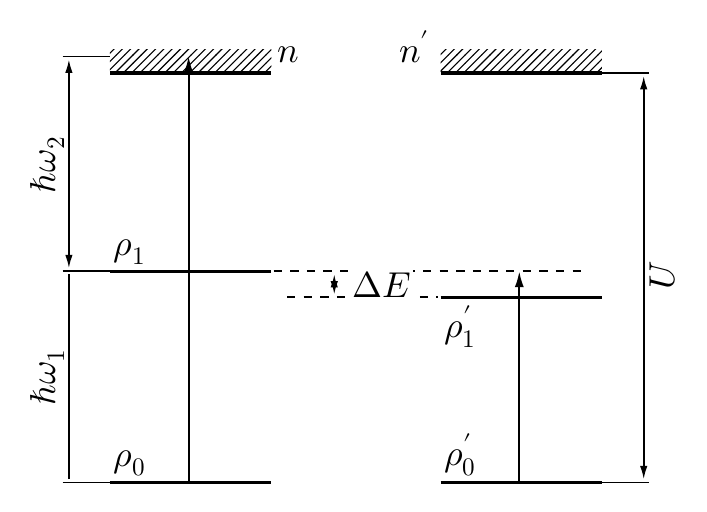
\begin{tikzpicture}[x=1cm,y=1cm]

% Schematic energies, not a numerical atomic spectrum.
\def\Eg{.45}\def\Ee{3.13}\def\Ep{2.80}\def\Eth{5.65}
\coordinate (g) at (2.0,\Eg);\coordinate (e) at (2.0,\Ee);
\coordinate (gp) at (6.2,\Eg);\coordinate (ep) at (6.2,\Ep);
\foreach \x in {1.0,5.2}{
 \draw[lev] (\x,\Eg)--++(2.05,0);
 \fill[pattern=north east lines,pattern color=Ink] (\x,\Eth) rectangle ++(2.05,.30);
 \draw[lev] (\x,\Eth)--++(2.05,0);
}
\draw[lev] (1.0,\Ee)--(3.05,\Ee) (5.2,\Ep)--(7.25,\Ep);
\draw[fine,dashed] (3.08,\Ee)--(7.08,\Ee) (3.25,\Ep)--(5.17,\Ep);
% A connected two-step path on the resonant isotope; no ionisation arrow at right.
\draw[ray] (g)--(2.0,5.86);
\draw[ray] (gp)--(6.2,\Ee);
\node[lab,anchor=south west] at (3.08,5.73) {$n$};
\node[lab,anchor=south east] at (5.12,5.73) {$n'$};
\node[lab,anchor=south west] at (1.0,.49) {$\rho_0$};
\node[lab,anchor=south west] at (1.0,3.17) {$\rho_1$};
\node[lab,anchor=south west] at (5.2,.49) {$\rho'_0$};
\node[lab,anchor=north west] at (5.2,2.74) {$\rho'_1$};
\draw[fine] (.40,\Eg)--(1,\Eg) (.40,\Ee)--(1,\Ee) (.40,5.86)--(1,5.86);
\draw[dim] (.48,.49)--(.48,3.09) (.48,3.17)--(.48,5.82);
\node[lab,rotate=90,fill=white] at (.21,1.79) {$\hbar\omega_1$};
\node[lab,rotate=90,fill=white] at (.21,4.49) {$\hbar\omega_2$};
\draw[fine] (7.25,\Eg)--(7.85,\Eg) (7.25,\Eth)--(7.85,\Eth);
\draw[dim] (7.78,.49)--(7.78,5.61);
\node[lab,rotate=90,fill=white] at (8.02,3.05) {$U$};
% External arrows: arrow tips touch the two gap boundaries, not empty space.
\draw[dim,line width=.70pt] (3.85,{\Ep+.035})--(3.85,{\Ee-.035});
\node[lab,anchor=west,fill=white,inner sep=1.4pt] at (4.03,2.96) {$\Delta E$};
\end{tikzpicture}
\end{document}
